\section{Preprocessing}
\subsection{Brainstorming Indicators}
Here are presented all the indicators that could be considered in a similar study.

\subsection{Screening the Indicators}
The second phase consists in finding problems with indicators, while they work on their own, they might expose problems with others or be irrelevant to the bigger picture. Several criteria are used and will be here presented one by one

\subsubsection{Availability of data}

\subsubsection{Double Counting}

\subsubsection{Irrelevant to the Decision Problem}

\subsection{Finalization of the Indicators}
Here is the final list and the aggregation

---
\textcolor{red}{EVERYTHING BELOW HAS TO BE REORGANIZED}


\section{Observation on the validity of public surveys}
During this study's execution, multiple public surveys were reviewed based on the initial assumption that such instruments could provide quantitative measurements of qualitative factors such as public support for nuclear installations. However, the analysis exposed frequent methodological limitations introducing bias into the results. In Italy, a 2024 survey reported 81\% opposition to nuclear power \cite{IPSOS_Nuclear_Survey_2024}. However, analysis of the survey report reveals problematic question design. The primary question was phrased as: \textit{"The debate on nuclear energy has returned to the forefront. What is your opinion on the matter?"} with response options structured as:
\begin{itemize}
    \item A1: "The current situation is complex; a return to nuclear should be evaluated"
    \item A2: "Nuclear has more risks than benefits and is not the right path"
    \item A3: "Nuclear energy entails excessive hidden costs and is not advantageous"
    \item A4: "Only safer technologies than current ones should be considered"
\end{itemize}

This framing demonstrates clear bias: two options (A2 and A3) explicitly oppose nuclear, A1 offers only conditional support, and A4 introduces safety concerns before suggesting potential support. Notably, the 81\% opposition figure includes A4 responses, which represent conditional rather than absolute opposition. When considering only explicit opposition (A2+A3), the figure decreases to 43\%.\\

Another study from 2024 presents a more methodologically sound approach, though its conference presentation emphasized positive findings. The actual data reveals a more nuanced picture: over 80\% of respondents consider themselves insufficiently informed about nuclear topics, and further investigation found that approximately 90\% were unaware of \glspl{smr} or Generation IV reactors \cite{SWG_Nuclear_Survey_2024}. These findings suggest that public opinion on nuclear energy may be more influenced by lack of information than by firmly held positions.

--justification for why we do not use surveys as indicator data...---

\subsection{Technical parameters}
The frist set of indicators are technical parameters that define the performance of each reactor design form an engineering standpoint.
An overview of technical parameters is presented in Table \ref{tab:indicators-technical}.
\paragraph{Thermal efficiency} indicates the fraction of thermal power generated by fission that is converted into net electrical power, accounting for in-plant consumption. Efficiency values were calculated using net electrical power output and thermal power data from the \gls{aris} database \cite{iaea2025aris}:
$$
\eta = \frac{P_{el,net}}{P_{th}}
$$
This indicator is a way to judge the thermal-hydraulic design of the reactor.

\paragraph{Discharge Burnup} measures the energy extracted per unit of heavy metal from the nuclear fuel ($MWd/tonHM$). Data for APR1400 and AP1000 were sourced from the \gls{aris} database \cite{iaea2025aris}, while EPR 1750 data were obtained from \cite{NRC_ML052280170}. Ranges are provided for SMRs due to design variability. Such value is indicative of the neutronics and core design of the reactor.

\paragraph{\gls{mox}} fuel is produced through spent nuclear fuel reprocessing and offers a solution for partially closing the nuclear fuel cycle in thermal reactors. While this process generates some secondary waste, it provides several strategic advantages: reducing final nuclear waste volumes, minimizing mining waste, and decreasing dependence on uranium imports. The latter is particularly relevant for Europe, which lacks significant domestic uranium deposits. However, reprocessing also presents proliferation risks since the extracted plutonium could potentially be diverted for weapons production. Due to these competing factors, nuclear fuel reprocessing is a fundamental strategic decision; the United States has foregone this practice, while France and UK have implemented the process in their nuclear programs \cite{CRS_Reprocessing_Spent_Fuel_2025}.

Given the European context of this study, MOX compatibility is considered a relevant reactor attribute. The evaluation methodology assigned each reactor design an initial score (0-10) based on its maximum MOX core fraction capability, followed by qualitative adjustments reflecting design-specific features. The complete scoring process and results are detailed in Table \ref{tab:mox-compatibility}.


\paragraph{Technological Readiness} of each reactor design was assessed by expert consultation by presenting them the current state of each design which...

\begin{table}[!ht]
    \centering
    \begin{tabularx}{\textwidth}{X c c c c}
        \toprule
        \textbf{Reactor Model} & \textbf{T1} & \textbf{T2} & \textbf{T3} & \textbf{T4}\\
        \midrule
        APR1400         & 35.2 & 46.5 & 3 & - \\
        EPR 1750        & 36.2 & 55 & 9 & -\\
        AP1000          & 32.4 & 50 & 6 & - \\
        BWRX-300        & 34.5 & $50 \pm 5$ & 0 & - \\
        Rolls Royce SMR & 34.6 & $55 \pm 5$ & 0 & - \\
        NuScale         & 30.8 & $52.5 \pm 2.5$ & 1 & - \\
        \bottomrule
    \end{tabularx}
    \caption{Technical Indicators: T1: Net efficiency [\%], T2: Discharge burnup [$MWd/tonHM$], T3: MOX fuel compatibility score, T4: Technological Readiness Level for selected reactor models}
    \label{tab:indicators-technical}
\end{table}


\begin{table}[!hb]
    \centering
    \begin{tabularx}{\textwidth}{l c X c c}
        \toprule
        \textbf{Reactor Model} & \textbf{MOX[\%]} & \textbf{Considerations} & \textbf{Score} & Sources \\
        \midrule
        APR1400         & 33 & - & 3/10 & \cite{iaea2025aris} \\
        \cmidrule(lr){1-5}
        EPR 1750        & 100 & 50\% without modifications, to reach 100\% "design adaptations which are not significantly costly" are required.  & 9/10 & \cite{iaea2025aris, osti_22257897} \\
        \cmidrule(lr){1-5}
        AP1000          & 50 & 50\% without modification, to reach 100\% major modifications are required & 6/10 & \cite{iaea2025aris, FETTERMAN2009324} \\
        \cmidrule(lr){1-5}
        BWRX-300        & 0 & GNF-2 Not manufactured with MOX & 0/10 & \cite{CNSC_BWRX300_Fuel_Design} \\
        \cmidrule(lr){1-5}
        Rolls Royce SMR & 0 & Rolls Royce states that they are not planning to use MOX & 0/10 & \cite{RollsRoyce_SMR_GDA_Consultation} \\
        \cmidrule(lr){1-5}
        NuScale         & 0 & Not licensing for MOX but a study reveals support is possible without design modifications & 1/10 & \cite{NRC_ML17007A001, NuScale_MOX_2016} \\
        \bottomrule
    \end{tabularx}
    \caption{MOX fuel compatibility scores and maximum MOX fraction}
    \label{tab:mox-compatibility}
\end{table}

\subsection{System parameters}
Two parameters were identified to characterize how the deployment of a reactor could fit into the existing grid of a country. The focus was on the ability to satisfy the peculiar demand of each country. The indicators are summarized in Table \ref{tab:indicators-system}.

\paragraph{Net Electric Power Output} has to be considered when choosing a power plant in relation to the needs of the local energy market, for instance a country that is constantly importing a substantial amount of energy might prefer large power plants rather then \glspl{smr}, on the other hand countries where renewable energy dominates the mix, small and flexible power could be preferred. For three large reactors data was sourced from \cite{IAEA_PRIS_2025} while for \glspl{smr} data was obtained from \cite{iaea2025aris}.


\paragraph{\glspl{lfc}} can be quantitatively assessed using characteristic curves that represent ramp-up and ramp-down rates as a function of load (expressed as percentage of nominal power $\%P_{nom}$), as illustrated in Figure \ref{fig:load-following-curve}. To facilitate comparative analysis, these performance curves are reduced to scalar values through integration of the area under said curve.

\begin{figure}[!hb]
    \centering
    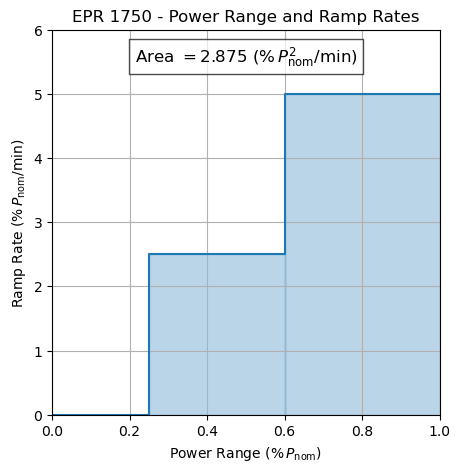
\includegraphics[width=0.7\textwidth]{imgs/load_following_curve.png}
    \caption{Example \gls{lfc} curve for EPR-1750}
    \label{fig:load-following-curve}
\end{figure}

For benchmarking purposes, the \gls{lfc} of a pair a tipical gas powered plant was computed. Specifically, a combined cyle plant featuring two heavy-duty GE Vernova 9HA.02 gas turbines (2015 data) \cite{GE_9HA_Gas_Turbine_2015}. 
Sources for load following data for APR1400, AP1000, BWRX-300 and Rolls Royce SMR where sourced from \cite{iaea2025aris}, while EPR 1750 data was obtained from \cite{OECD_NEA_Load_Following_2011}. For NuScale data was sourced from \cite{ENCO_SMR_Analysis_2022}.

\begin{table}[!ht]
    \centering
    \begin{tabularx}{0.6\textwidth}{l X X}
        \toprule
        \textbf{Reactor Model} & \textbf{S1} & \textbf{S2}\\
        \midrule
        APR1400           & 1340 & 0.21 \\
        EPR 1750          & 1630 & 2.88 \\
        AP1000            & 1120 & 4.25 \\
        BWRX-300          & 300 & 0.25 \\
        Rolls Royce SMR   & 470 & 2.00 \\
        NuScale (Voygr-6) & 462  & 2.00 \\
        GE 9HA.02 2xCC    & 1515 & 7.02 \\
        \bottomrule
    \end{tabularx}
    \caption{System Indicators: S1: Net Electric Power Output [$MW_{e,net}$], S2: \gls{lfc} [$\%P_{nom}/min$]}
    \label{tab:indicators-system}
\end{table}

\subsection{Economic Indicators}
Economic indicators are crucial in evaluating the feasibility and attractiveness of nuclear reactor designs. They provide insights into the financial implications of deploying and operating these technologies. The selected economic indicators are summarized in Table \ref{tab:indicators-economic}. To provide a reference the same indicators were also sourced for three renewable energy technologies: onshore wind, solar pv with battery storage and hydroelectric power \cite{EIA_Capital_Costs_AEO2024}. The commissioning time estimates fro solar and wind were taken from \cite{GUMBER2024122563} which also notes that the average (reported in our table) is significantly higher then the median, we choose to report the average since we deem it more representative of large installations.

\paragraph{Capital Costs} represent the initial investment required to construct a nuclear power plant. For this indicator we are going to present both the \glspl{noak} estimates as well as forecases or data for \gls{foak} installation. It is important to note that, as detailed by Rothwell 2022 \cite{ROTHWELL2022112905} the costs of recent nuclear installations in Europe and the US have been significantly higher than those announced at the start of the project. For this reason we will apply a FOAK-to-NOAK factor to better represent the real costs. For example the EPR-1600 announced costs for Flamanville-3 was 1886 $USD_{2020}/kW_e$ but have risen to 8600 $USD_{2020}/kW_e$ \cite{NEA2020}. All Values are summarized in Table \ref{tab:capital-costs}. \\

We want to clarify that the data has all been converted to 2020 USD since the main source of data \cite{STEIGERWALD2023128204} and \cite{NEA2020} reports all costs in this currency and year. \\

\paragraph{Commissioning Time} follows similar considerations to the previous paragraph, recent nuclear installations have suffered significant delays during construction. To esemplify this we will report both the planned commissioning time as well as the last unit commissioning time for each design. Information on three large reactors comes from \cite{nea2020unlocking} while estimates for the three \glspl{smr} come from manufacturer claims or related documents \cite{GEVernova_Nuclear_2025, RollsRoyce_SMR_Approach_2025, IEEFA_UAMPS_Talking_Points_2023}.

\paragraph{Operational Costs} are ongoing expenses incurred during the operation and maintenance of a nuclear power plant. These costs encompass fuel expenses, routine maintenance and etc. Steigerwald et al. (2023) \cite{STEIGERWALD2023128204} provides comprehensive cost analyses for future nuclear installations, including capital and operational expenditures for both SMRs and large reactors. The study reports operational costs in $USD_{2020}/MWh_e$ for EPR and APR1400 designs, as well as a "Long-Term US" category which this analysis uses as AP1000 costs. For SMRs, operational costs were originally presented in power-based units ($USD_{2020}/MW_e$), requiring conversion to energy-based measurements ($USD_{2020}/MWh_e$) using a Gaussian distribution of capacity factors ($\mu$ = 90\%, $\sigma$ = 5\%) according to:

$$
\frac{USD_{2020}}{MWh_e} = \frac{USD_{2020}}{MW_e} \cdot \frac{1}{CF \cdot 8760 \frac{h}{year}}
$$

The same study reports fuel costs of $6.23 USD_{2020}/MWh_e$ for PWR-based technologies with the exceptions of NuScale at $7.15 USD_{2020}/MWh_e$ and the only BWR reactor at $29.55 USD_{2020}/MWh_e$. For comparative context, operational cost estimates for utility-scale onshore wind, hydroelectric, and solar PV (with single axis tracking and DC battery storage) were obtained from the U.S. Energy Information Administration \cite{EIA_Capital_Costs_AEO2024}. All cost data have been standardized to 2020 USD to maintain consistency with the primary data sources \cite{STEIGERWALD2023128204, NEA2020}, values are presented in Table \ref{tab:operational-costs}.

\begin{table}[!hb]
    \centering
    \begin{tabularx}{\textwidth}{X c c c c c}
        \toprule
        \textbf{Reactor Model} & \textbf{E1} & \textbf{E2} & \textbf{E3} & \textbf{E4} & \textbf{E5} \\
        \midrule
        APR-1400         & 2410 & 1828 & 18.44 & 5.0 (KOR) & 10 and 8 in (KOR) \\
        EPR-1750        & 8600 & 2150 & 14.26 & 5.0 (EU) 4.5 (CN) & 9 (CN), 17 (EU) \\
        AP-1000          & 8600 & 2000 & 18.69 & 5.0 (US) & 9 (CN), 10, 11 (US) \\
        BWRX-300        & 3467 & 2318 & $18.30 \pm 0.82$ & $2.5 \pm 0.5$ & NA \\
        Rolls Royce SMR & 7408 & 6050 & $65.68 \pm 2.94$ & 4.0 & NA \\
        NuScale         & 8600 & 3466 & $22.76 \pm 1.02$ & 4.0 & NA \\
        \textbf{Other Power Plants} & & & & & \\
        Onshore Wind   & NA & 1265 & 28.08 & NA & 2.7 \\
        Solar PV + Battery & NA & 2175 & 33.33 & NA & 2.3 \\
        Hydroelectric  & NA & 6007 & 28.49 & NA & PLACEHOLDER \\
        \bottomrule
    \end{tabularx}
    \caption{Economic Indicators E1-E5: E1: Capital costs for FOAK installations [\$/kWe], E2: Capital costs for NOAK installations [\$/kWe], E3: Operational costs [\$/MWh], E4: Planned commissioning time [years], E5: Real building times [years]}
    \label{tab:consolidated-costs-building-time}
\end{table}


\paragraph{Potential Impact on the energy market} can be estiated by...

\subsection{Indicators on Social Matters}
\paragraph{Potential Reduction of \glspl{ghg}} were quantified by comparing each country's 2024 emissions against projected emissions following deployment of one reactor unit. Country-specific GHG emission intensities were derived from Electricity Maps aggregated data \cite{ElectricityMaps_CarbonIntensity_2024}. Total load were obtained from the ENTSO-E Transparency Platform \cite{ENTSOE_Transparency_2025}. Due to non-normal data distributions, median values with interquartile ranges were employed to characterize uncertainty (Table~\ref{tab:ghg-intensity-country}). \\

For nuclear generation's lifecycle emissions, Liu et al.'s (2023) comprehensive meta-analysis of 42 studies \cite{10.3389/fenrg.2023.1147016} served as the primary reference, reporting a global average of $15.815 \pm 3.59 \; gCO_{2,\text{eq}}/kWh_e$ for light water reactors. This conservative estimate was selected despite lower values observed in specific contexts: French nuclear operations typically range between $ 2 \sim 6 \; gCO_{2,\text{eq}}/kWh_e$ according to both operational data \cite{paillere_2021} and IAEA assessments \cite{IAEA_Climate_Change_Nuclear_Power_2022}, while individual studies on french reactors have reported values as high as $12 \; gCO_{2,\text{eq}}/kWh_e$ \cite{paillere_2021}. The global average was preferred to account for potential regional variations in fuel cycle practices and construction impacts. \\

Small modular reactors (SMRs) were assigned an emission intensity of $17.24 \pm 3.91$ $gCO_{2,\text{eq}}/kWh_e$, incorporating Carless et al.'s (2016) finding that SMRs exhibit approximately $9\%$ higher lifecycle emissions than conventional large LWRs due to reduced economies of scale in construction and fuel production \cite{CARLESS201684}. \\

\begin{table}[!ht]
    \centering
    \begin{tabularx}{0.6\textwidth}{X c c c}
        \toprule
        Country / Region & a & b & c \\
        \midrule
        Italy (IT)        & draft & 240 & 72.0 \\
        Switzerland (CH)  & 60  & draft  & 1.8 \\
        Poland (PL)       & 160 & 700 & draft \\
        France (FR)       & 460 & draft  & 23.0 \\
        \bottomrule
    \end{tabularx}
    \caption{\gls{ghg} evaluation: a: Annual electricity load [TWh], b: GHG emission intensity [gCO$_2$-eq/kWh], c: Total annual GHG emissions from electricity generation [MtCO$_2$-eq/yr]}
    \label{tab:ghg-intensity-country}
\end{table}



\paragraph{Spent Nuclear Fuel Production} was estimated based on...

\paragraph{Mining Waste} are estimated ....

\paragraph{Percived Safety}
The observant reader may have noted the omission of explicit safety indicators among technical parameters in our analysis. Table~\ref{tab:safety-performance} presents a critical regulatory metric. How is the Core Damage Frequency (CDF) calculated and validated by nuclear regulators: the Core Damage Frequency (CDF), representing the probabilistic assessment of severe accident likelihood, expressed as events leading to core damage per reactor-year.

\begin{table}[!ht]
    \centering
    \begin{tabularx}{\textwidth}{X c c}
        \toprule
        \textbf{Reactor Model} & \textbf{CDF [1/reactor-year]} & Source\\
        \midrule
        APR-1400         & $2.25 \times 10^{-6}$ & \cite{KHNP_EU_APR_Characteristics} \\
        EPR-1750         & $1.18 \times 10^{-7}$ & \cite{EDFEnergy_PSA_2012} \\
        AP1000           & $2.41 \times 10^{-7}$ & \cite{NRC_ML23161A411} \\
        BWRX-300         & $<1.0 \times 10^{-8}$ & \cite{ENCO_SMR_Analysis_2022} \\
        Rolls-Royce SMR  & $<1.0 \times 10^{-7}$ & \cite{ENCO_SMR_Analysis_2022} \\
        NuScale          & $<2.0 \times 10^{-7}$ & \cite{ENCO_SMR_Analysis_2022} \\
        \bottomrule
    \end{tabularx}
    \caption{Core Damage Frequency (CDF) for Selected Reactor Models}
    \label{tab:safety-performance}
\end{table}

While CDF values demonstrate marginal differences between designs, all modern reactors exhibit exceptionally high safety performance in absolute terms. Comparative energy safety data underscores this point: nuclear energy's fatality rate of 0.03 deaths per TWh places it among the safest energy sources, comparable to wind (0.04) and solar (0.02), and 2-3 orders of magnitude safer than fossil fuels (2.82 for gas, 32.72 for brown coal) \cite{Markandya_Wilkinson_2007, SOVACOOL20163952, OurWorldInData_EnergyDeathRates_2025}. Radiation exposure data from the U.S. EPA \cite{EPA_Radiation_Sources_2025}, based on NCRP measurements \cite{NCRP_Report_160_2009}, reveals that 48\% of average annual radiation dose comes from medical procedures, 37\% originates from natural background radiation and less than 0.2\% is attributable to occupational/industrial sources, including nuclear power plants.

\text{orange}{MAYBE OMIT: Notably, as first documented by McBride et al. (1978) \cite{McBride_Radiological_Impact_1978}, coal plants typically emit radioactive materials at levels two orders of magnitude higher than nuclear plants when normalized for equivalent energy production.}

Therefore, considering the following:
\begin{itemize}
    \item All evaluated reactors meet comparable, high safety standards
    \item Nuclear energy demonstrates superior safety performance relative to conventional energy sources
    \item Technical safety metrics have limited influence on public perception and reactor preference, where risk perception often diverges from actual risk assessment
\end{itemize}

The safety indicator will not be based on risk assessment data but will be derived from expert judgment based on the percived risk that each reactor model may present to the general public.
